\subsection{Спектральный анализ}
Спектральный анализ - это один из методов обработки сигналов, который позволяет охарактеризовать частотный состав измеряемого сигнала.
Методы статистики играют важную роль в спектральном анализе, поскольку сигналы, как правило, имеют шумовой или случайный характер. Если бы
основные статистические характеристики сигнала были известны точно или же их можно было бы без ошибок определить на конечном интервале этого
сигнала, то спектральный анализ представлял бы собой отрасль точной науки. В действительности по одному-единственному отрезку сигнала можно
получить только некоторую оценку его спектра. Практика спектрального анализа после 1880-х гг. постепенно стала превращаться в некое ремесло
достаточно субъективного характера, которое на ряду с использованием научного подхода требовало также определенного уровня эмпирического
искусства \cite{marpl_book}.

\subsubsection{Применение нормального уравнения Юла-Уокера}
В 1927 г. Дж. Юл предложил существенно новый метод спектрального анализа. Для отыскания одной-двух периодичностей в исследуемых данных Юл
прибег к моделированию временного ряда, основанному на линейном регрессионном анализе. Юла интересовала главным образом более высокая точность
определения основной периодичности в ряде чисел солнечных пятен и отыскания в нем дополнительных периодичностей \cite{marpl_book}.
Используя простое тригонометрическое тождество:
\begin{center}
\begin{equation}
	\label{eq:yule_trigonometric}
	\sin(kx)=2\cos(x)\sin([k-1]x)-sin([k-2]x)
\end{equation}
\end{center}
Используя подстановки и обобщая формулу (весь ход обобщения описан в \cite{marpl_book}) можно получить:
\begin{center}
\begin{equation}
	\label{eq:yule_raznost}
	u(k) = a(1)u(k-1) + a(2)u(k-2) + \epsilon (k)
\end{equation}
\end{center}
Здесь ${u(k) = \sin (2\pi fkT)}$ - гармоническая составляющая, ${T}$ - интервал отсчетов, ${f}$ - частота гармоники,
${\epsilon (k)}$ - некоторое малое импульсное возмущение, а ${a(1)}$ и ${a(2)}$ принимают произвольные значения.
Как легко увидеть, уравнение \ref{eq:yule_raznost} представляет собой АР уравнение. Юл предположил, что
если процесс имеет только один тон, то он может быть описан как \ref{eq:yule_raznost}.
Решением уравнения \ref{eq:yule_raznost} является затухающая синусоида.

АР модель предсказания отсчета может быть описана как взвешенная сумма ${P}$ предыдущих отсчетов сигнала:
\begin{center}
\begin{equation}
	\label{eq:lpc_forecast}
	\hat{x}(m) = \sum \limits_{k=1}^P a_k x(m-k),
\end{equation}
\end{center}
где ${\hat{x}(m)}$ - оценка ${x(m)}$ в момент времени ${m}$, а ${a_k}$ - коэффициенты АР-модели, ${P}$ - порядок модели.

Специфичной для детектирования ШПС является необходимость определения точной фазы ПСП
для работы с сигналом. Так же при обработке ШПС от нескольких источников с разными ПСП необходимо учитывать,
что оценка спектра будет смещенной и требуется его корректировка. После повторной модуляции
с синхронизированной копией ПСП получается гармоническая компонента на промежуточной частоте и шум. Подробнее компоненты шума были
рассмотрены в \ref{l:noise_model}. Преобразуем выражение \ref{eq:gps_signal_modulated}: амплитуду гармонического
сигнала возьмем ${A = 1}$, ${D_k(t)}$ примем за 1, учитывая, что мы оцениваем параметры сигнала в пределах одной
ПСП:
\begin{center}
\begin{equation}
	\label{eq:lpc_signal}
	x(t) = \cos(\omega_{c}t + \phi(t)) + n(t)
\end{equation}
\end{center}

Для уравнения \ref{eq:lpc_signal}, необходимо записать ковариации для 3 точек
${r_{xx}(0)}$, ${r_{xx}(1)}$, ${r_{xx}(2)}$:

\begin{center}
\begin{equation}
	\label{eq:lpc_cov}
	{r_{xx}(\tau) = \frac{1}{N} \sum \limits_{n=0}^{N-1} x(n) x(n-\tau)}
\end{equation}
\end{center}

Для применения АР метода является очень существенным знать модель шумовой компоненты ${n(t)}$ из выражения
\ref{eq:lpc_signal}. Зная АКФ ${n(t)}$, можно получить несмещенную оценку ${\omega_c}$.

Ошибка предсказания ${e(m)}$ может быть представлена как:
\begin{center}
\begin{equation}
	\label{eq:lpc_error}
	e(m) = x(m) - \hat{x}(m) = x(m) - \sum \limits_{k=1}^P a_k x(m-k),
\end{equation}
\end{center}

Из уравнения \ref{eq:lpc_error} смоделированный сигнал может быть представлен следующим рекурсивным соотношением:
\begin{center}
\begin{equation}
	\label{eq:lpc_signal}
	x(m) = \sum \limits_{k=1}^P a_k x(m-k) + e(m)
\end{equation}
\end{center}

Уравнение \ref{eq:lpc_error} представляет собой цифровой фильтр.
После ${z}$ - преобразования уравнение \ref{eq:lpc_signal} может быть записано как \cite{saeed_book}:
\begin{center}
\begin{eqnarray}
	\label{eq:lpc_z}
		H(z)	& = & \frac{X(z)}{U(z)} = \frac{G}{1 - \sum \limits_{k=1}^P a_kz^{-k}} =  \nonumber \\
			& = & G\frac{1}{\prod \limits_{k=1}^N (1-r_kz^{-1})} \frac{1}{\prod \limits_{k=1}^M (1-2r_k \cos \phi_k z^{-1} + r_k^2z^{-2})}
\end{eqnarray}
\end{center}

В уравнении \ref{eq:lpc_z} ${M}$ - пар комплексных полюсов, ${N}$ - действительные полюсы с ${P=N+2M}$,
${r_k}$ и ${\phi_k}$ - радиус и угол ${k}$ - го полюса соответственно. Частотный ответ такой системы 
может быть представлен \cite{saeed_book}:
\begin{center}
\begin{eqnarray}
	\label{eq:lpc_freq_resp}
		H(f)	& = & = \frac{G}{1 - \sum \limits_{k=1}^P a_k e^{-j2 \pi kf}} =  \nonumber \\
			& = & G\frac{1}{\prod \limits_{k=1}^N (1-r_k e^{-j2 \pi f)}} \frac{1}{\prod \limits_{k=1}^M (1-2r_k \cos \phi_k e^{-j2 \pi f} + r_k^2 e^{-j4 \pi f})}
\end{eqnarray}
\end{center}

Уравнения, соответствующие линейному предсказанию, по своей структуре идентичны уравнениям Юла-Уокера для АР-процесса.
В виду этого существует тесная связь между фильтром линейного предсказания и АР-процессом \cite{marpl_book}.

На рисунке \ref{pic:lpc_poles} изображено отношение между полюсами и АЧХ рекурсивного фильтра. На частотах, соответствующих полюсам,
на графике АЧХ присутствуют частотные пики. Пары комплексных корней могут быть представлены через радиус ${r_k}$ и угол ${\phi_k}$
полюса:
\begin{center}
\begin{equation}
	\label{eq:lpc_poles}
	z_k = r_k e^{\pm j \phi_k}
\end{equation}
\end{center}

Для определения резонансной частоты ${H(z)}$ можно воспользоваться формулой:
\begin{center}
\begin{equation}
	\label{eq:lpc_poles_freq}
	\omega_k = arg(z_k)
\end{equation}
\end{center}

\begin{figure}[H]
	\center\scalebox{1}{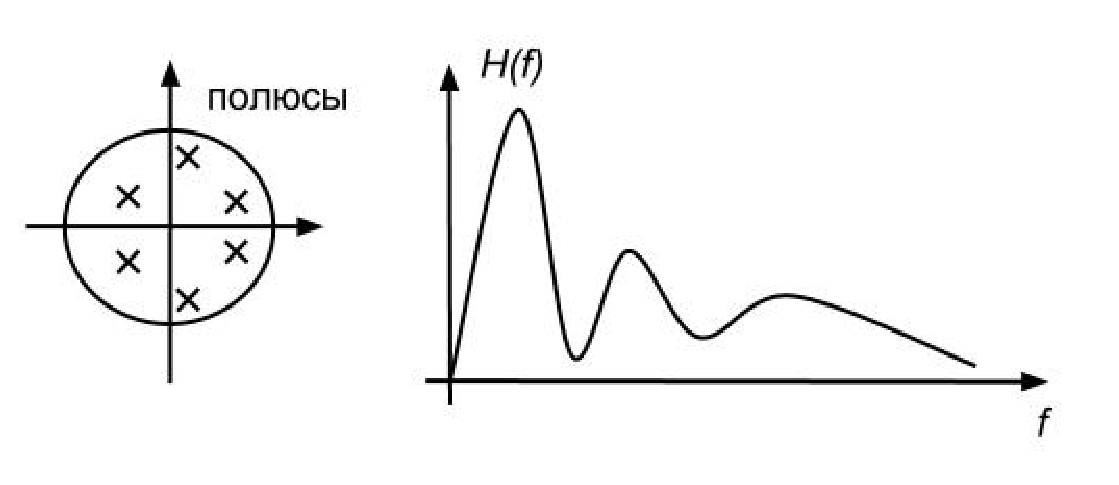
\includegraphics[width=1\linewidth]{lpc_poles.eps}}
	\caption{Полюса и АЧХ линейного предсказателя}
	\label{pic:lpc_poles}
\end{figure}

\paragraph{Вычисление коэффициентов АР модели}
Наилучшие оценки коэффициентов ${a_k}$ могут быть получены минимизацией среднеквадратичной ошибки уравнения \cite{saeed_book} \ref{eq:lpc_error}:

\begin{center}
\begin{eqnarray}
	\label{eq:lpc_rms}
		E[e^2(m)]	& = & E[(x(m) - \sum \limits_{k=1}^P a_k x(m-k))^2] =\nonumber \\
				& = & E[x^2(m)] - \nonumber \\
				& &  - 2\sum \limits_{k=1}^P a_k E[x(m-k)x(m)] + \nonumber \\
				& &  + \sum \limits_{k=1}^P a_k \sum \limits_{j=1}^P a_j E[x(m-k)x(m-j)] = \nonumber \\
				& = & r_{xx}(0) - 2{\bf r}^T_{xx}{\bf a} + {\bf a}^T {\bf R_{xx}a}
\end{eqnarray}
\end{center}
где ${{\bf R_{xx}} = E[{\bf xx}^T]}$ - это автокорреляционная матрица входного вектора \\
${{\bf x}^T=[x(m-1),x(m-2),...,x(m-P)]}$,
${{\bf r}_{xx}=E[x(m){\bf x}]}$ - автокорреляционный вектор, а ${a^T=[a_1,a_2,...,a_P]}$ -  вектор коэффициентов предсказателя.
Минимизация среднеквадратичной ошибки из уравнения \ref{eq:lpc_rms} может быть записано как:
\begin{center}
\begin{equation}
	\label{eq:lpc_rms2}
	{\bf a=R^{-1}_{xx}r_{xx}}
\end{equation}
\end{center}
где матрица ${\bf R_{xx}}$ является тёплицевой и эрмитовой, поскольку  ${r_{xx}(-k) = r_{xx}(k)}$. Данная
процедура является реализацией алгоритма Юла-Уокера. В данном алгоритме предполагается, что истинные значения
АКП ${r_{xx}(k)}$ известны. На практике значения АКП не известны и их приходится заменять оценкой ${\hat{r}_{xx}(k)}$, что может
при несмещенных оценках ${\hat{r}_{xx}(k)}$ привести к не положительно определенной матрице ${\bf {R_{xx}}}$, а значит
к неустойчивой АР модели \cite{bolshakov-book}.

В случае вычисления параметров АР модели путем решения уравнений Юла-Уокера, нахождение полюсов
внутри единичной окружности не очевидно. В \cite{shahtarin-spectrum-book} показано, что если
автокорреляционная матрица  ${{\bf R_{xx}}}$ является положительно определенной, то и решение
линейных уравнений Юла-Уокера порождает устойчивый чисто полюсный фильтр.

При больших объемах выборки входных данных алгоритм Юла-Уокера дает вполне приемлемые результаты, в то время
как при малых выборках оценки параметров дают СПМ с низкой разрешающей способностью \cite{marpl_book, bolshakov-book}.

Можно использовать альтернативную запись.  Для сигнала длинной в ${N}$ семплов можно записать ${N}$ - уравнений:
\begin{center}
\begin{equation}
	\label{eq:lpc_rms3}
	{\bf e=x-Xa}
\end{equation}
\end{center}
Уравнение \ref{eq:lpc_rms3} можно переписать в виде:
\begin{center}
\begin{equation}
	\label{eq:lpc_rms4}
	{\bf e^T e = xx^T - 2x^T Xa + a^T X^T Xa}
\end{equation}
\end{center}

Взяв производную по вектору ${{\bf a}}$, можно получить параметры предсказателя:
\begin{center}
\begin{equation}
	\label{eq:lpc_rms5}
	\frac{\partial {\bf e^T e}}{\partial {\bf a}} = {\bf - 2x^T X + a^T X^T X} = 0
\end{equation}
\end{center}
Из \ref{eq:lpc_rms6}, коэффициенты для минимальной среднеквадратичной ошибки равны:
\begin{center}
\begin{equation}
	\label{eq:lpc_rms6}
	{\bf a= (X^T X)^{-1} (X^T x)}
\end{equation}
\end{center}

Из сравнения уравнений \ref{eq:lpc_rms2} и \ref{eq:lpc_rms6} видно, что в \ref{eq:lpc_rms2}
автокорреляционная матрица и вектор заменены оценками:
\begin{center}
\begin{equation}
	\label{eq:lpc_rxx_estimation}
	\hat{r}_{xx}(m) = \frac{1}{N} \sum \limits_{k=0}^{N-1} x(k)x(k-m)
\end{equation}
\end{center}

Для решения уравнения Юла-Уокера можно применить метод Гаусса, а так же его модификации: LU-разложение,
разложение Холецкого, UD-разложение. Данные методы требуют выполнения вычислительных операций, пропорционально ${P^3}$.
Но так  как \ref{eq:lpc_rms2} является тёплицевой и эрмитовой, можно использовать эффективные методы работы
с тёплицевыми матрицами, которые значительно лучше упомянутых выше. 
Например, можно воспользоваться, быстрым алгоритмом Левинсона-Дарби.
Быстрым алгоритмам над тёплицевыми матрицами посвящена книга \cite{bleyhut_book}.

АР метод оценки СПМ часто используется для того, чтобы выявить в данных наличие синусоидальных
компонент. Мощность, соответствующую  таким компонентам в АР оценке СПМ, можно вычислить, интегрируя
площадь под кривой этой оценки. Однако это связано с большими вычислительными затратами, поэтому
гораздо более эффективным является использования в качестве показателя мощности синусоидальных
компонент высоты соответствующих им спектральных пиков \cite{marpl_book}.  

%%%%%%%%%%%%%%%%%%%%%%%%%%%%%%%%%%%%%%%%%%%%%%%%%%%%%%%%%%%%%%
\subsubsection{АР модель второго порядка. Оценка частоты основного тона на основе АР-модели}

АР-модель второго порядка применяется для определения частоты основного тона. Для поиска единственного
тона необходимо найти 2 полюса. Тогда выражение \ref{eq:lpc_rms2} может быть записано как:
\begin{center}
\begin{equation}
	\label{eq:lpc_a_estimation}
	\left[ \begin{array}{c}
		\hat{a}_1 \\
		\hat{a}_2
	\end{array} \right]
	=
		\left[ \begin{array}{cc}
			r_{xx}(0)  + \sigma_n^2 & r_{xx}(1)\\
			r_{xx}^*(1) & r_{xx}(0) + \sigma_n^2 
		\end{array} \right]^{-1}
		\left[ \begin{array}{c}
			r_{xx}(1) \\
			r_{xx}(2)
		\end{array} \right]
	= \bf{R_x^{-1}r_{xx}}
\end{equation}
\end{center}

Здесь ${\hat{a}_1, \hat{a}_2}$, - МНК оценки коэффициентов АР-модели, ${r_{xx}(m)}$ - АКФ принимаемого сигнала.
Для оценки АКФ  можно использовать выражение \ref{eq:lpc_rxx_estimation}:

Передаточная функция АР-модели второго порядка ${H(z)}$:
\begin{center}
\begin{equation}
	\label{eq:lpc_spectral_func}
	H(z) = \frac{1}{1 - a_1 z^{-1} - a_2 z^{-2}}
\end{equation}
\end{center}

Характеристическое уравнение
\begin{center}
\begin{equation}
	\label{eq:lpc_characteristic}
	z^2 - a_1 z - a_2 = 0
\end{equation}
\end{center}
имеет полюсы
\begin{center}
\begin{equation}
	\label{eq:lpc_poles_2}
	z_{1,2} =\frac{a_1 \pm \sqrt{a_1^2 + 4 a_2}}{2}
\end{equation}
\end{center}

Для определения резонансной частоты ${H(z)}$ можно воспользоваться формулой \ref{eq:lpc_poles_freq}.
Для принятия решения о наличии гармонического сигнала анализируют значение квадрата модуля частотной
характеристики АР-модели в точке резонанса:
\begin{center}
\begin{equation}
	\label{eq:lpc_power_cos}
	\left| H(z) \right|^2 = \frac{1}{\left| 1 - a_1 e^{-j \omega_0} - a_2 e^{-2 \omega_0} \right|^2}
\end{equation}
\end{center}

Если это значение превышает некоторый заранее выбранный порог, то принимается решение о наличии гармонического
сигнала с частотой ${\omega_0}$. 

%%%%%%%%%%%%%%%%%%%%%%%%%%%%%%%%%%%%%%%%%%%%%%%%%%%%%%%%%%%%%%
\subsubsection{Использование АР-модели для детектирования ШПС}
\label{ssec2:lpc_cdma_detect}

При работе с ПСП следует учитывать, что после демодуляции входного сигнала выровненной ПСП в сигнале восстанавливается 1 гармоническая
компонента, что дает возможность использовать АР-модель второго порядка.
Повторная модуляция сигнала с ПСП по любой фазе отличной от искомой не будет восстанавливать гармонический сигнал.
Спектр гармонического сигнала повторно модулированного ПСП с не выровненной фазой будет такой же, как у исходного сигнала – отображен
на рисунке \ref{pic:lpc_psd_1} штриховой пунктирной линией. И только повторная модуляция с выровненной фазой ПСП даст спектр
изображенный красной линией на рисунке \ref{pic:lpc_psd_1}.

На \ref{pic:lpc_basic1} входной сигнал повторно модулируется ПСП с известной фазой.

\begin{figure}[H]
	\center\scalebox{0.8}{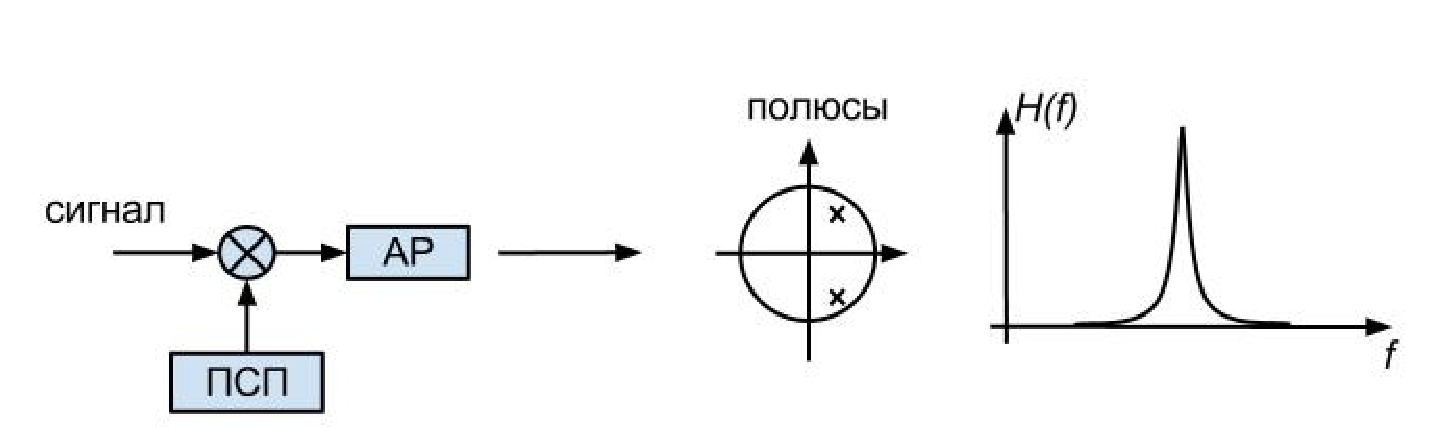
\includegraphics[width=1\linewidth]{lpc_basic.eps}}
	\caption{Общая схема применения АР-модели для детектирования ШПС сигнала}
	\label{pic:lpc_basic1}
\end{figure}

Выходом алгоритма будет СПМ, а пик будет соответствовать энергии на определенной частоте. На рисунке
\ref{pic:lpc_poles_gps} красным изображена энергия гармонического колебания с большой мощностью, а
зеленым изображен цветной шум.
\begin{figure}[H]
	\center\scalebox{1}{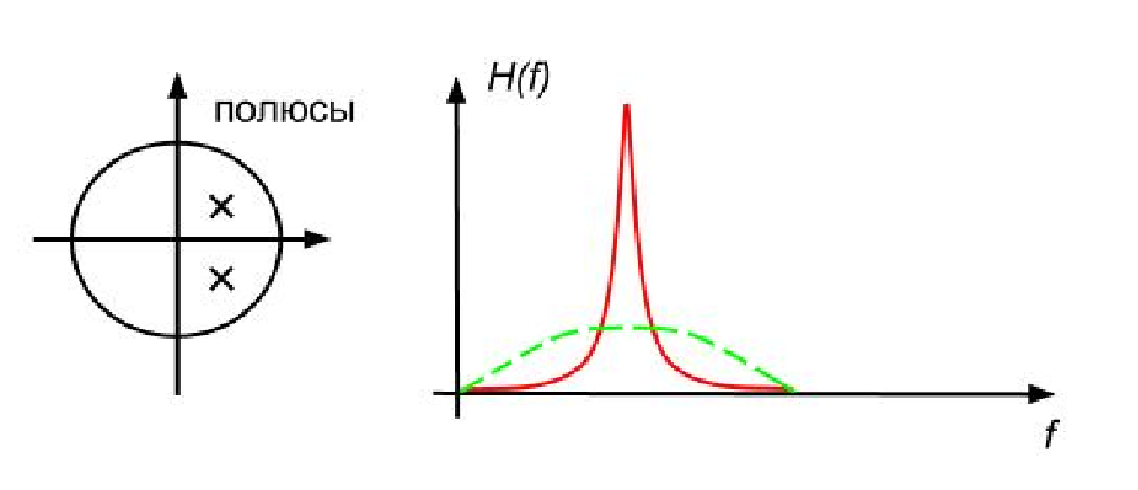
\includegraphics[width=1\linewidth]{lpc_poles_gps.eps}}
	\caption{Полюс и АЧХ линейного предсказателя}
	\label{pic:lpc_poles_gps}
\end{figure}

Так же необходимо отметить, что фаза ПСП в момент начала приема сигнала не известна.
Для оценки частоты сигнала необходимо для каждой фазы ПСП вычислить квадрат частотного
отклика.

Описанный алгоритм состоит из следующих шагов(${\tau \in [0, \tau_{max}]}$):
\begin{itemize}
\item[Шаг 1.] Вычисляются оценки АКФ в трех точках (для аргументов АКФ=0,1,2)
	для фазы ПСП ${\tau}$ по формуле \ref{eq:lpc_rxx_estimation}. 
\item[Шаг 2.] Определяются коэффициенты АР-модели ${\hat{a_1}, \hat{a_2}}$, 
	по формуле \ref{eq:lpc_a_estimation}. 
	Вычисляется резонансная частота ${\omega_0}$ по формуле \ref{eq:lpc_poles_freq}
	и определяется квадрат модуля частотного отклика АР-модели для этой частоты по выражению \ref{eq:lpc_power_cos}. 
\item[Шаг 3.] Полученное значение квадрата частотного отклика сравнивается с заранее выбранным порогом детектора. 
	\subitem{\bf{Если}}  значение оказалось больше порогового {\bf{то}} 
		принимается решение о наличии сигнала, а в качестве оценки
		частоты принимается значение ${\omega_0}$ соответствующее смещению ПСП равному ${\tau}$. 
	\subitem{\bf{Иначе если}} ${\tau}$ меньше длины ПСП ${\tau = \tau + 1}$ и переход к шагу 1.
	\subitem{\bf{Иначе}} 
		Принимается решение об отсутствии гармонического сигнала.
\end{itemize}

%%%%%%%%%%%%%%%%%%%%%%%%%%%%%%%%%%%%%%%%%%%%%%%%%%%%%%%%%%%%%%
\subsubsection{Влияние теплового шума на точность оценки частоты с помощью АР-модели}
Серьезным фактором ограничивающим применение АР-модели при оценке параметров гармонического сигнала является
его чувствительность к тепловому шуму. Разрешающая способность оценки
частоты при применении АР-модели снижается при снижении уровня ОСШ - выражение \ref{eq:lpc_est_quality_1}.
В \cite{kay_ar_book} приведены ссылки на работы
\cite{lacoss_spectral_est, chen_spectral_est, marple_1977} подтверждающие данное поведение.

Различные методы оценки параметров для АР-модели основанные на принципе максимального правдоподобия больше не
могут считаться ММП при наличии шума в данных. В виду сложности использования ММП, предложено несколько 
субоптимальных оценок \cite{marpl_book, kay_ar_book}:
\begin{enumerate}
	\item Применение АРСС;
	\item Фильтрация данных для уменьшения мощности шума;
	\item Компенсация параметров АР или оценки коэффициентов отражения;
	\item Использования АР-модели более высокого порядка.
\end{enumerate}

Разрешение оценки АР-модели для гармонических сигналов одинаковой мощности в случае известной АКФ
можно определить приблизительно с помощью формулы Марпла \cite{marpl_book, kay_ar_book}:
\begin{center}
\begin{equation}
	\label{eq:lpc_est_quality_1}
	F = \frac{1.03}{Tp[SNR(p+1)]^{0.31}}
\end{equation}
\end{center}

где ${F}$ - разрешение в герцах, T - интервал отсчетов в секундах, ${p}$ - порядок модели,
${SNR}$ - ОСШ для отдельного гармонического сигнала, выраженный в линейных единицах.

Поскольку порядок модели в нашем случае 2, выражение \ref{eq:lpc_est_quality_1} можно переписать:
\begin{center}
\begin{equation}
	\label{eq:lpc_est_quality_2}
	F = \frac{0.36635}{SNR^{0.31}}
\end{equation}
\end{center}

Соотношение \ref{eq:lpc_est_quality_2} позволяет оценить точность разрешения синусоидальной компоненты
для заданного значения ОСШ, что необходимо для оценки допустимости величины входной расстройки частоты.
Большое значение входной расстройки ведет к необходимости увеличения входной полосы ФАПЧ, а это
отрицательно сказывается на рабочих характеристиках модуля ФАПЧ.

\newpage
